\documentclass[14pt]{extbook}
\usepackage{multicol, enumerate, enumitem, hyperref, color, soul, setspace, parskip, fancyhdr} %General Packages
\usepackage{amssymb, amsthm, amsmath, latexsym, units, mathtools} %Math Packages
\everymath{\displaystyle} %All math in Display Style
% Packages with additional options
\usepackage[headsep=0.5cm,headheight=12pt, left=1 in,right= 1 in,top= 1 in,bottom= 1 in]{geometry}
\usepackage[usenames,dvipsnames]{xcolor}
\usepackage{dashrule}  % Package to use the command below to create lines between items
\newcommand{\litem}[1]{\item#1\hspace*{-1cm}\rule{\textwidth}{0.4pt}}
\pagestyle{fancy}
\lhead{Progress Quiz 6}
\chead{}
\rhead{Version A}
\lfoot{4563-7456}
\cfoot{}
\rfoot{Summer C 2021}
\begin{document}

\begin{enumerate}
\litem{
Solve the radical equation below. Then, choose the interval(s) that the solution(s) belongs to.\[ \sqrt{-3 x + 7} - \sqrt{8 x + 8} = 0 \]\begin{enumerate}[label=\Alph*.]
\item \( \text{All solutions lead to invalid or complex values in the equation.} \)
\item \( x_1 \in [-2.89, -0.37] \text{ and } x_2 \in [0.33,4.33] \)
\item \( x \in [1.09,1.63] \)
\item \( x \in [-0.53,0.06] \)
\item \( x_1 \in [-0.53, 0.06] \text{ and } x_2 \in [0.33,4.33] \)

\end{enumerate} }
\litem{
What is the domain of the function below?\[ f(x) = \sqrt[7]{8 x + 9} \]\begin{enumerate}[label=\Alph*.]
\item \( (-\infty, \infty) \)
\item \( \text{The domain is } [a, \infty), \text{   where } a \in [-1.67, -1.11] \)
\item \( \text{The domain is } (-\infty, a], \text{   where } a \in [-2.68, -0.99] \)
\item \( \text{The domain is } [a, \infty), \text{   where } a \in [-0.9, -0.84] \)
\item \( \text{The domain is } (-\infty, a], \text{   where } a \in [-0.98, 0.99] \)

\end{enumerate} }
\litem{
Solve the radical equation below. Then, choose the interval(s) that the solution(s) belongs to.\[ \sqrt{-63 x^2 - 32} - \sqrt{92 x} = 0 \]\begin{enumerate}[label=\Alph*.]
\item \( x \in [-0.73,-0.31] \)
\item \( x_1 \in [-0.92, -0.72] \text{ and } x_2 \in [-2.57,0.43] \)
\item \( \text{All solutions lead to invalid or complex values in the equation.} \)
\item \( x_1 \in [0.74, 1.27] \text{ and } x_2 \in [-0.43,2.57] \)
\item \( x \in [-0.92,-0.72] \)

\end{enumerate} }
\litem{
Choose the graph of the equation below.\[ f(x) = - \sqrt[3]{x - 6} + 7 \]\begin{enumerate}[label=\Alph*.]
\begin{multicols}{2}\item 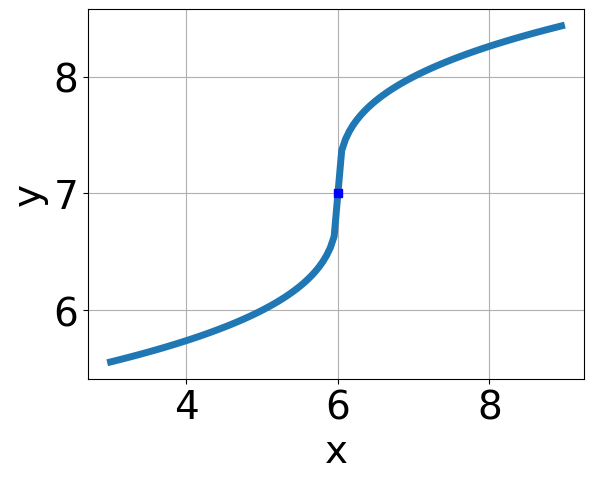
\includegraphics[width = 0.3\textwidth]{../Figures/radicalEquationToGraphAA.png}\item 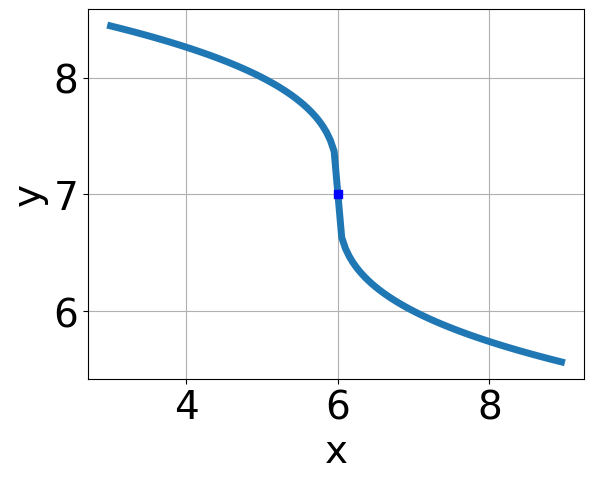
\includegraphics[width = 0.3\textwidth]{../Figures/radicalEquationToGraphBA.png}\item 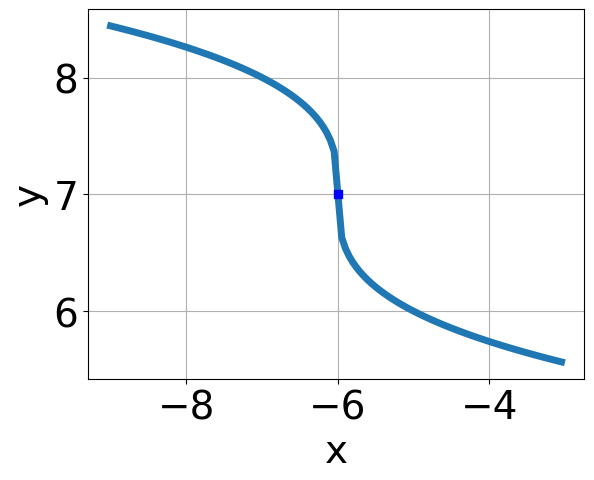
\includegraphics[width = 0.3\textwidth]{../Figures/radicalEquationToGraphCA.png}\item 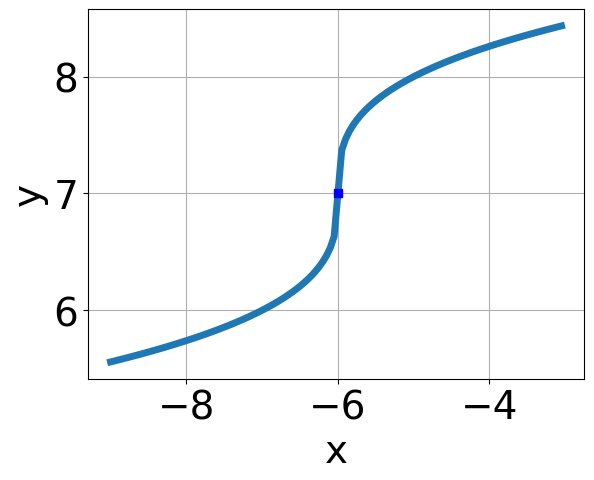
\includegraphics[width = 0.3\textwidth]{../Figures/radicalEquationToGraphDA.png}\end{multicols}\item None of the above.
\end{enumerate} }
\litem{
Solve the radical equation below. Then, choose the interval(s) that the solution(s) belongs to.\[ \sqrt{-15 x^2 - 24} - \sqrt{49 x} = 0 \]\begin{enumerate}[label=\Alph*.]
\item \( x_1 \in [-3.5, -1.4] \text{ and } x_2 \in [-1.6,0.4] \)
\item \( x \in [-3.5,-1.4] \)
\item \( x \in [-1.2,-0.3] \)
\item \( \text{All solutions lead to invalid or complex values in the equation.} \)
\item \( x_1 \in [1.7, 5.2] \text{ and } x_2 \in [-0.4,4.6] \)

\end{enumerate} }
\litem{
Choose the equation of the function graphed below.
\begin{center}
    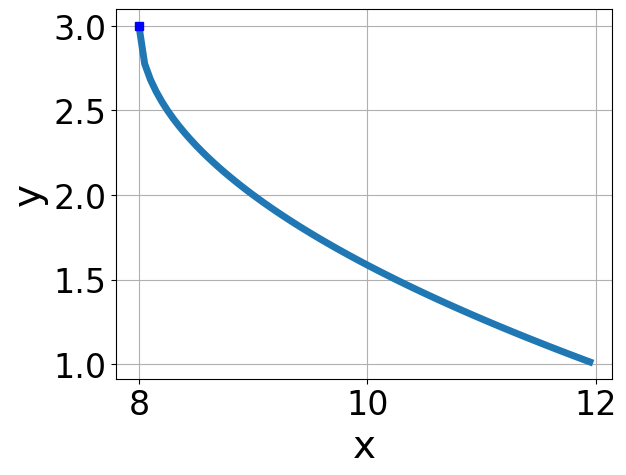
\includegraphics[width=0.5\textwidth]{../Figures/radicalGraphToEquationCopyA.png}
\end{center}
\begin{enumerate}[label=\Alph*.]
\item \( f(x) = \sqrt{x - 8} + 3 \)
\item \( f(x) = - \sqrt{x - 8} + 3 \)
\item \( f(x) = - \sqrt{x + 8} + 3 \)
\item \( f(x) = \sqrt{x + 8} + 3 \)
\item \( \text{None of the above} \)

\end{enumerate} }
\litem{
Choose the graph of the equation below.\[ f(x) = - \sqrt{x + 8} - 4 \]\begin{enumerate}[label=\Alph*.]
\begin{multicols}{2}\item 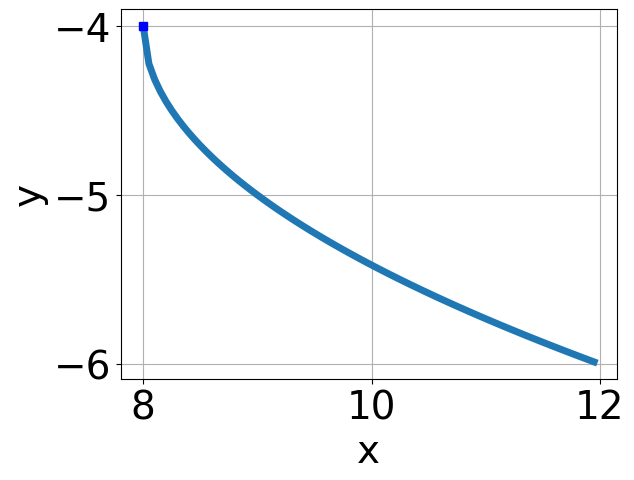
\includegraphics[width = 0.3\textwidth]{../Figures/radicalEquationToGraphCopyAA.png}\item 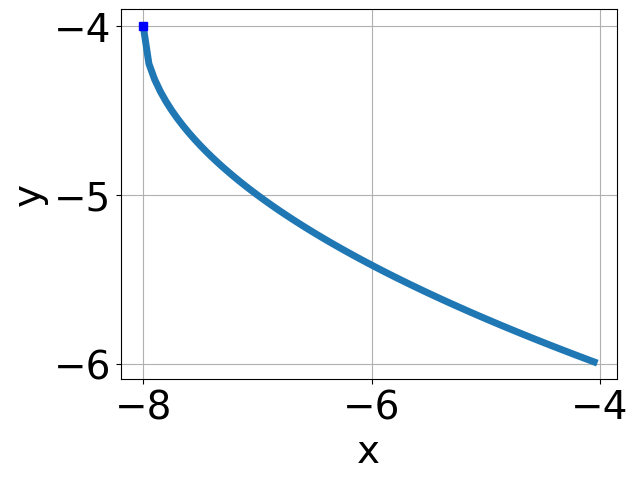
\includegraphics[width = 0.3\textwidth]{../Figures/radicalEquationToGraphCopyBA.png}\item 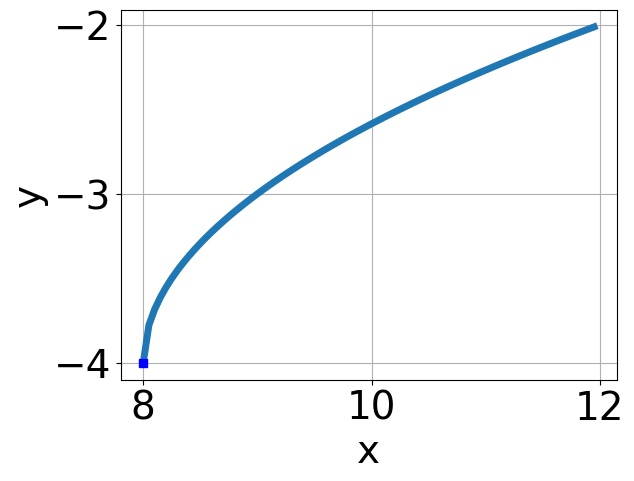
\includegraphics[width = 0.3\textwidth]{../Figures/radicalEquationToGraphCopyCA.png}\item 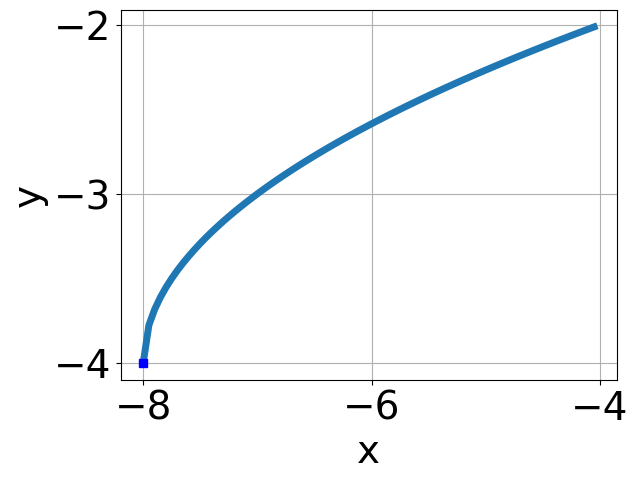
\includegraphics[width = 0.3\textwidth]{../Figures/radicalEquationToGraphCopyDA.png}\end{multicols}\item None of the above.
\end{enumerate} }
\litem{
Choose the equation of the function graphed below.
\begin{center}
    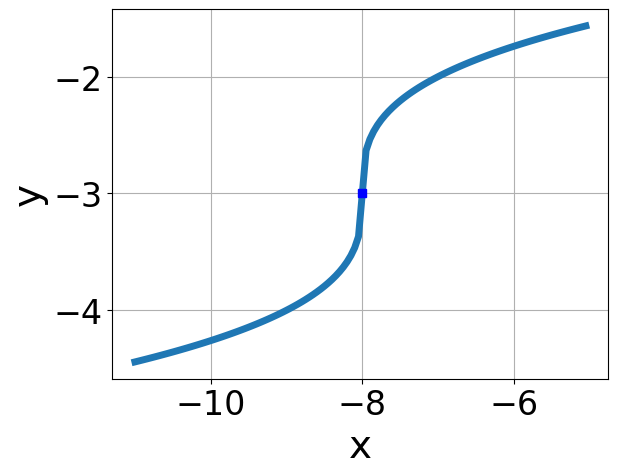
\includegraphics[width=0.5\textwidth]{../Figures/radicalGraphToEquationA.png}
\end{center}
\begin{enumerate}[label=\Alph*.]
\item \( f(x) = \sqrt{x + 8} - 3 \)
\item \( f(x) = - \sqrt{x - 8} - 3 \)
\item \( f(x) = \sqrt{x - 8} - 3 \)
\item \( f(x) = - \sqrt{x + 8} - 3 \)
\item \( \text{None of the above} \)

\end{enumerate} }
\litem{
What is the domain of the function below?\[ f(x) = \sqrt[6]{5 x - 8} \]\begin{enumerate}[label=\Alph*.]
\item \( (-\infty, \infty) \)
\item \( [a, \infty), \text{where } a \in [-0.57, 0.71] \)
\item \( (-\infty, a], \text{where } a \in [1, 1.75] \)
\item \( [a, \infty), \text{ where } a \in [0.88, 2.21] \)
\item \( (-\infty, a], \text{where } a \in [0.56, 1.32] \)

\end{enumerate} }
\litem{
Solve the radical equation below. Then, choose the interval(s) that the solution(s) belongs to.\[ \sqrt{-6 x - 5} - \sqrt{9 x - 4} = 0 \]\begin{enumerate}[label=\Alph*.]
\item \( x \in [-0.47,0.01] \)
\item \( x \in [-0.63,-0.23] \)
\item \( x_1 \in [-0.87, -0.76] \text{ and } x_2 \in [0.25,0.5] \)
\item \( \text{All solutions lead to invalid or complex values in the equation.} \)
\item \( x_1 \in [-0.87, -0.76] \text{ and } x_2 \in [-1.44,0.22] \)

\end{enumerate} }
\end{enumerate}

\end{document}